\chapter{Introduction}
\vspace{-1cm}
\epigraphfontsize{\small\itshape}
\epigraph{“...if we were to name the most powerful assumption of all, which leads one on
and on in an attempt to understand life, it is that all things are made of atoms, and
that everything that living things do can be understood in terms of the jigglings and
wigglings of atoms.”}
{--- \textup{Richard P. Feynman}, The Feynman Lectures on Physics\cite{feynmanLectures}}

\section{Deoxyribonucleic Acid}

\section{Polymer Physics}

\newpage

\section{Computer Simulations}

The theory of classical mechanics is regarded as the first major breakthrough in the
field of physics. For every aspiring physicist this is still the starting point of their
studies. Unfortunately getting to know these relatively simple laws of nature, leads to
the inescapable realisation that these theories are expressed in mathematical formalism
that are only analytically solvable in few idealised scenarios. Already when trying to
apply these formulas to a problem consisting of just more then two bodies the equations
become practically unsolvable, this fact has vexed physicists and mathematician for many
years.\\


\begin{wrapfigure}{r}{0.5\textwidth}
  \begin{center}
    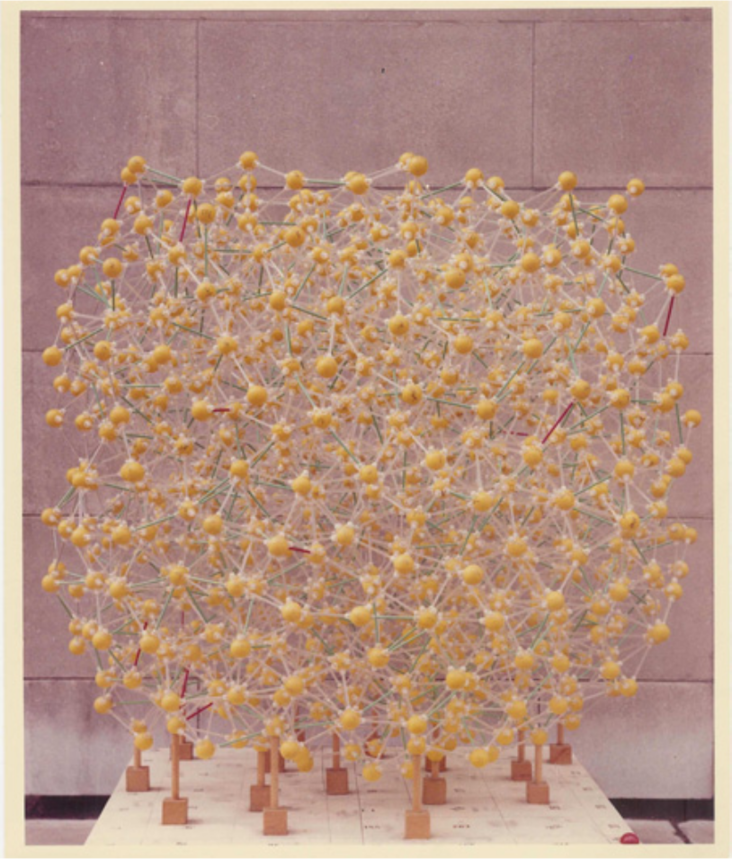
\includegraphics[width=0.48\textwidth]{Figures/WaterModel.png}
  \end{center}
  \caption{Example of an expanded model of a simple liquid (J L Finney, Ph.D thesis)}
\end{wrapfigure}


Although it is often times not possible to find an exact solution to many equations
encountered in physics, finding reasonable approximations to their solution is. Various
types of
techniques are used to find these approximations, ranging from taylor expansions to
simulations.
Before the invention of computers these simulations where performed mechanical and
consisted of large amounts of

 \begin{quote}
\dots I took a number of rubber balls and stuck them together with rods of a
selection of different lengths ranging from 2.75 to 4 inch. I tried to do this in the
first place as casually as possible, working in my own office being interrupted every
five minutes or so and not remembering what I had done before the interruption.
However,\dots
\end{quote}

mechanical simulations -> bernal

computer simulations -> los alamos, fast adaptation by industry.

Biophysics / consedmatter physics, many body systems, bridge between the micro scopic and
macro scopic


\subsection{Molecular Dynamics Simulations}
Molecular Dynamics Simulations (MD) is a computer simulation techniques used to analyse
the dynamics of a classical many-body system. In a system with $N$ particles the motion



The central idea is that
the trajectories of a system of $N$ particles can be generated over time by numerically
integrating the classical equations of motion.




- Iterating Newton laws of physics
\[
    m_i \boldsymbol{\ddot{r_i}} = \boldsymbol{f_i}, \quad \boldsymbol{f_i} = -
    \frac{\partial}{\partial \boldsymbol{r_i}} \mathcal{U}
\]
- thermostats

- Integrations schemes

- Rare event sampling

\begin{algorithm}
    \SetKwFunction{isOddNumber}{isOddNumber}
    \SetKwInOut{KwIn}{Input}
    \SetKwInOut{KwOut}{Output}

    \KwIn{Configuration of the system at $t=0$}
    \KwOut{Configuration of the system at $t=t_{f}$}

    $newList = [\ ]$

    \tcc{For odd elements in the list, we add 1, and for even elements, we add 2.
    After the loop, all elements are even.}
    \For{$i \leftarrow 0$ \KwTo $n-1$}{
        \eIf{$\isOddNumber(a_i)$}{

            $newList.append(a_i + 1)$ \tcp*[f]{Some thought-provoking comment.}
         }{
            \tcp{Another comment}
            $newList.append(a_i + 2)$
         }
    }

    \KwRet{$newList$}
    \caption{The Velocity Verlet algorithm}
\end{algorithm}

% \begin{center}
% 	\begin{tikzpicture}[
% 	squarednode/.style={rectangle, draw=blue!60, fill=blue!5, very thick, minimum width=50mm,
% 	minimum height=5mm},]
% 	%Nodes
% 	\node[squarednode]      (step1)                        {1};
% 	\node[squarednode]      (step2)       [below= 3mm of step1] {2};
% 	\node[squarednode]      (step3)       [below= 3mm of step2] {3};
% 	\node[squarednode]      (step4)       [below= 3mm of step3] {4};
% 	\node[squarednode]      (step5)       [below= 3mm of step4] {5};
% 	\node[squarednode]      (step6)       [below= 3mm of step5] {6};
% 	\node[squarednode]      (step7)       [below= 3mm of step6] {7};
% 	\node[squarednode]      (step8)       [below= 3mm of step7] {8};
%
% 	%Lines
%     \draw[very thick, ->] (step1.south) -- (step2.north);
% 	\draw[very thick, ->] (step2.south) -- (step3.north);
% 	\draw[very thick, ->] (step3.south) -- (step4.north);
% 	\draw[very thick, ->] (step4.south) -- (step5.north);
%     \draw[very thick, ->] (step5.south) -- (step6.north);
% 	\draw[very thick, ->] (step6.south) -- (step7.north);
% 	\draw[very thick, ->] (step7.south) -- (step8.north);
% 	\draw[very thick, ->] (step8.west)  -- +(-0.4,0) |-(step2.west);
% 	\end{tikzpicture}
% \end{center}

- understanding many body - newtons algorithm
- insight in the dynamics -> simulate trajectories
- recent developments in techniques to simulate trajectories of rare event
-increased computational power
\subsection{Coarse Grained modelling}
